\chapter{कोशिका का उपापचय}\label{ch:g10:cell-metabolism}

गुनगुने चीनी वाले पानी की एक फ़्लास्क में एक चम्मच पावरोटी वाला खमीर
डालिए और उसकी गरदन पर एक गुब्बारा चढ़ा दीजिए। घंटे भर में तरल धुँधला
होकर बुलबुले छोड़ने लगता है, गुब्बारा तनकर खड़ा हो जाता है, और फ़्लास्क
से हल्की-सी ब्रेड और बियर जैसी गंध आती है। खमीर की \omterm{def:g10:cells-common-unit:cell}{कोशिकाएँ} चीनी खा रही
हैं और उसे किसी और चीज़ में बदल रही हैं, और वे जो गैस छोड़ती हैं वह वही
कार्बन डाइऑक्साइड है जिसे आप साँस के साथ बाहर निकालते हैं। धूप में रखा
कोई पत्ता उल्टा करता है: वह कार्बन डाइऑक्साइड भीतर लेता है और ऑक्सीजन
बाहर देता है। दोनों रसायन ही हैं, जो \omterm{def:g10:cells-common-unit:cell}{कोशिकाओं} के भीतर, शरीर के ताप पर,
बिना किसी लौ और बिना किसी अम्ल के चलता है --- और यह अध्याय उसी रसायन के
बारे में है।

\section{उपापचय: कोशिका का रसायन}

\begin{definition}[उपापचय]\label{def:g10:cell-metabolism:metabolism}
किसी \omterm{def:g10:cells-common-unit:cell}{कोशिका} का \emph{उपापचय}\index{उपापचय} उन सभी रासायनिक अभिक्रियाओं
का समुच्चय है जो उसके भीतर चलती हैं: वे भी जो ऊर्जा छोड़ने के लिए अणुओं
को तोड़ती हैं, और वे भी जो सरल अणुओं से \omterm{def:g10:cells-common-unit:cell}{कोशिका} के अपने अणु बनाती हैं।
उपापचय की हर अभिक्रिया को कोई \emph{एंजाइम}\index{एंजाइम} चलाता है, यानी
ऐसा \omterm{def:g10:chemistry-of-life:families}{प्रोटीन} जो किसी एक विशिष्ट अभिक्रिया को तेज़ करता है पर ख़ुद उसमें
ख़र्च नहीं होता।
\end{definition}

\begin{proposition}[एंजाइम ही कोशिका का रसायन संभव बनाते हैं]\label{prop:g10:cell-metabolism:enzymes}
\qty{37}{\celsius} पर हवा में पड़ा ग्लूकोज़ जलता नहीं; \omterm{def:g10:cells-common-unit:cell}{कोशिका} में वह
कुछ ही मिनटों में पूरा ऑक्सीकृत हो जाता है। फ़र्क़ एंजाइमों का है: हर
\omterm{def:g10:cell-metabolism:metabolism}{एंजाइम} किसी ख़ास अणु (अपने \emph{क्रियाधार}) से जुड़ता है, उसे उत्पाद
में बदलता है, छोड़ देता है और फिर शुरू हो जाता है --- हर सेकंड हज़ारों
बार। इसलिए किसी \omterm{def:g10:cells-common-unit:cell}{कोशिका} का \omterm{def:g10:cell-metabolism:metabolism}{उपापचय} उसके पास मौजूद एंजाइमों के समुच्चय से तय
होता है --- और वह समुच्चय उसके \omterm{def:g10:universal-dna:gene}{जीनों} से।
\end{proposition}
\admitted

\begin{example}[एक एंजाइम काम पर]\label{ex:g10:cell-metabolism:catalase}
कच्चे यकृत या आलू के टुकड़े पर हाइड्रोजन परॉक्साइड डालिए: ऑक्सीजन छूटते
ही वह ज़ोर से झाग उठता है। \omterm{def:g10:cell-metabolism:metabolism}{एंजाइम} कैटेलेज़, जो लगभग हर \omterm{def:g10:cells-common-unit:cell}{कोशिका} में है,
विषैले परॉक्साइड को जल और ऑक्सीजन में तोड़ता है --- प्रति \omterm{def:g10:cell-metabolism:metabolism}{एंजाइम} अणु
प्रति सेकंड लाखों अणुओं की दर से। यकृत को पहले उबाल दीजिए तो कुछ नहीं
होता: वह \omterm{def:g10:cell-metabolism:metabolism}{एंजाइम}, जो एक \omterm{def:g10:chemistry-of-life:families}{प्रोटीन} है, ऊष्मा से नष्ट हो चुका है। और पत्थर पर
डाला गया परॉक्साइड बिना बुलबुलों के पड़ा रहता है, जो दिखाता है कि
अभिक्रिया अपने आप नहीं चलती।
\end{example}

\begin{omfigure}
\begin{tikzpicture}[>=Stealth, font=\small]
  \node[draw, rounded corners, fill=omDef!15, minimum width=1.6cm, minimum height=1.1cm] (e1) at (0,0) {एंजाइम};
  \node[draw, fill=omProp!30, minimum width=0.9cm, minimum height=0.5cm] (s) at (0,1.3) {क्रियाधार};
  \draw[->] (s) -- (e1);
  \node[draw, rounded corners, fill=omDef!15, minimum width=1.6cm, minimum height=1.1cm] (e2) at (4,0) {एंजाइम};
  \node[draw, fill=omProp!30, minimum width=0.9cm, minimum height=0.5cm, anchor=south] (s2) at (4,0.55) {क्रियाधार};
  \draw[->] (e1.east) -- node[above] {जुड़ता है} (e2.west);
  \node[draw, rounded corners, fill=omDef!15, minimum width=1.6cm, minimum height=1.1cm] (e3) at (8,0) {एंजाइम};
  \node[draw, fill=omMeth!30, minimum width=0.5cm, minimum height=0.5cm] (p1) at (7.5,1.5) {उत्पाद};
  \node[draw, fill=omMeth!30, minimum width=0.5cm, minimum height=0.5cm] (p2) at (9.1,1.5) {उत्पाद};
  \draw[->] (e2.east) -- node[above] {बदलता है} (e3.west);
  \draw[->] (e3.north) -- (p1.south);
  \draw[->] (e3.north) -- (p2.south);
  \draw[->, dashed] (e3.south) to[bend left=25] node[below] {अनबदला छूटता है, फिर शुरू} (e1.south);
\end{tikzpicture}

{\small कोई \omterm{def:g10:cell-metabolism:metabolism}{एंजाइम} अपने क्रियाधार से जुड़ता है, उसे बदलता है और उत्पाद
छोड़ देता है, जबकि ख़ुद अनबदला रहता है। \omterm{def:g10:cell-metabolism:metabolism}{एंजाइम} का एक अणु यह चक्र हर सेकंड
हज़ारों बार दोहरा सकता है।}
\end{omfigure}

\section{कोशिका को खिलाने के दो रास्ते}

\begin{definition}[स्वपोषण और परपोषण]\label{def:g10:cell-metabolism:autotrophy}
कोई \omterm{def:g10:cells-common-unit:cell}{कोशिका} \emph{स्वपोषी}\index{स्वपोषण} है यदि वह अपने कार्बनिक अणु
अकेले \omterm{def:g10:chemistry-of-life:mineral-organic}{खनिज पदार्थ} से --- कार्बन डाइऑक्साइड, जल, \omterm{def:g10:chemistry-of-life:mineral-organic}{खनिज लवण} से --- किसी
बाहरी ऊर्जा-स्रोत की मदद से बना ले। \omterm{def:g10:cells-common-unit:organelle}{हरितलवक} वाली पादप \omterm{def:g10:cells-common-unit:cell}{कोशिकाएँ}, शैवाल और
कुछ जीवाणु स्वपोषी हैं, और उनका ऊर्जा-स्रोत प्रकाश है: यही
\emph{प्रकाशसंश्लेषण}\index{प्रकाशसंश्लेषण} है। कोई \omterm{def:g10:cells-common-unit:cell}{कोशिका}
\emph{परपोषी}\index{परपोषण} है यदि उसे दूसरे जीवों के बनाए कार्बनिक अणु
भीतर लेने ही पड़ें, निर्माण-सामग्री के रूप में भी और ऊर्जा के स्रोत के
रूप में भी: जंतु \omterm{def:g10:cells-common-unit:cell}{कोशिकाएँ}, कवक, अधिकांश जीवाणु, और पौधों की बिना हरे रंग
वाली \omterm{def:g10:cells-common-unit:cell}{कोशिकाएँ} (जैसे जड़ों की) परपोषी हैं।
\end{definition}

\begin{proposition}[प्रकाशसंश्लेषण]\label{prop:g10:cell-metabolism:photosynthesis}
प्रकाश में \omterm{def:g10:cells-common-unit:organelle}{हरितलवक} वाली \omterm{def:g10:cells-common-unit:cell}{कोशिका} कार्बन डाइऑक्साइड और जल सोखती है,
ऑक्सीजन छोड़ती है, और ग्लूकोज़ बनाती है, जिसे वह आगे मंड, सेलुलोज़,
\omterm{def:g10:chemistry-of-life:families}{लिपिड} और खनिज नाइट्रोजन के साथ \omterm{def:g10:chemistry-of-life:families}{ऐमीनो अम्लों} में बदल देती है। संक्षेप
में:
\[
6\,\mathrm{CO_2} + 6\,\mathrm{H_2O} \xrightarrow{\ \text{प्रकाश, पर्णहरित}\ }
\mathrm{C_6H_{12}O_6} + 6\,\mathrm{O_2}.
\]
प्रकाश की ऊर्जा ग्लूकोज़ के रासायनिक बंधों में संचित हो जाती है।
\end{proposition}
\begin{proof}[साक्ष्य]
ऑक्सीजन संवेदक लगे किसी बंद पात्र में हरी शैवाल \emph{Chlorella} का
निलंबन दिखाता है कि लैंप जलने पर घुली हुई ऑक्सीजन लगातार बढ़ती है और
बुझने पर घटती है; और यदि पानी की कार्बन डाइऑक्साइड निकाल दी जाए तो बढ़ना
रुक जाता है। दो दिन अँधेरे में रखे पत्ते आयोडीन से नीले-काले नहीं होते,
और आधा पन्नी से ढँका पत्ता केवल अपने खुले आधे हिस्से पर रंग पकड़ता है:
मंड वहीं बनता है जहाँ प्रकाश पड़ता है। किसी पौधे को दी गई रेडियोसक्रिय
कार्बन डाइऑक्साइड कुछ ही मिनटों में उसकी शर्कराओं में जा पहुँचती है।
\end{proof}

\begin{omfigure}
\begin{tikzpicture}
\begin{axis}[
  width=0.88\linewidth, height=5.4cm,
  axis x line=bottom, axis y line=left,
  xmin=0, xmax=22, ymin=5, ymax=13,
  xlabel={समय (\unit{min})}, ylabel={घुली $\mathrm{O_2}$ (\unit{mg/L})},
  xlabel style={font=\small, at={(axis description cs:0.5,-0.12)}, anchor=north},
  ylabel style={font=\small},
  tick label style={font=\small}, xtick={0,5,10,15,20},
  clip=false,
]
\addplot[thick, omMeth] coordinates {(0,8.0) (5,8.0) (10,10.5) (15,10.0) (20,12.5)};
\draw[dashed, gray] (axis cs:5,5) -- (axis cs:5,13);
\draw[dashed, gray] (axis cs:10,5) -- (axis cs:10,13);
\draw[dashed, gray] (axis cs:15,5) -- (axis cs:15,13);
\node[font=\small, anchor=south] at (axis cs:2.5,12.5) {अँधेरा};
\node[font=\small, anchor=south] at (axis cs:7.5,12.5) {प्रकाश};
\node[font=\small, anchor=south] at (axis cs:12.5,12.5) {अँधेरा};
\node[font=\small, anchor=south] at (axis cs:17.5,12.5) {प्रकाश};
\end{axis}
\end{tikzpicture}

{\small किसी बंद \emph{Chlorella} निलंबन में घुली हुई ऑक्सीजन। प्रकाश
में शैवाल ऑक्सीजन को खपाने से तेज़ी से छोड़ती हैं; अँधेरे में केवल उनका
श्वसन बचता है और ऑक्सीजन गिरती है। हर ढाल एक दर है, जिसे मिलीग्राम प्रति
लीटर प्रति मिनट में पढ़ा जा सकता है।}
\end{omfigure}

\begin{example}[युग्लीना, एक साथ दोनों]\label{ex:g10:cell-metabolism:euglena}
एककोशिकीय \emph{Euglena} में \omterm{def:g10:cells-common-unit:organelle}{हरितलवक} होते हैं और वह एक कशाभिका से तैरती
है। प्रकाश में, खनिज जल में वह बढ़ती है: यानी \omterm{def:g10:cell-metabolism:autotrophy}{स्वपोषी}। अँधेरे में वह तभी
बची रहती है जब पानी में कार्बनिक अणु मिलाए जाएँ, जिन्हें वह सोख लेती है:
यानी \omterm{def:g10:cell-metabolism:autotrophy}{परपोषी}। लंबे समय तक अँधेरे में रखने पर वह अपने \omterm{def:g10:cells-common-unit:organelle}{हरितलवक} खो देती है;
और कुछ दिनों के धीरज के साथ प्रकाश में लौटाने पर वह उन्हें दोबारा बना
लेती है। उसका \omterm{def:g10:cell-metabolism:metabolism}{उपापचय} उसके \omterm{def:g10:universal-dna:gene}{जीनों} पर निर्भर है, जो दोनों विकल्प खुले रखते
हैं, और उसके पर्यावरण पर, जो उनमें से एक चुन लेता है।
\end{example}

\section{कार्बनिक अणुओं से ऊर्जा पाना}

\begin{proposition}[कोशिकीय श्वसन]\label{prop:g10:cell-metabolism:respiration}
हर \omterm{def:g10:cells-common-unit:cell}{कोशिका}, चाहे \omterm{def:g10:cell-metabolism:autotrophy}{स्वपोषी} हो या \omterm{def:g10:cell-metabolism:autotrophy}{परपोषी}, काम में आने वाली ऊर्जा कार्बनिक
अणुओं को तोड़कर ही पाती है। ऑक्सीजन उपलब्ध हो तो तोड़ना पूरा होता है ---
यही \emph{कोशिकीय श्वसन}\index{कोशिकीय श्वसन} है, जो \omterm{def:g10:cells-common-unit:organelle}{सूत्रकणिकाओं} में
चलता है:
\[
\mathrm{C_6H_{12}O_6} + 6\,\mathrm{O_2} \longrightarrow
6\,\mathrm{CO_2} + 6\,\mathrm{H_2O} + \text{ऊर्जा},
\]
यानी प्रति मोल ग्लूकोज़ (\qty{180}{g}) लगभग \qty{2870}{kJ}, जिसका मोटे
तौर पर 40\% एक छोटे अणु \emph{ATP}\index{ATP} में पकड़ लिया जाता है, और
\omterm{def:g10:cells-common-unit:cell}{कोशिका} की हर ऊर्जा माँगने वाली प्रक्रिया --- गति, परिवहन, संश्लेषण ---
उसी से खींचती है; बाक़ी ऊष्मा के रूप में छूट जाता है।
\end{proposition}
\begin{proof}[साक्ष्य]
ऑक्सीजन संवेदक लगे बंद पात्र में भूखा खमीर कोई ऑक्सीजन नहीं खपाता;
ग्लूकोज़ मिलाइए तो घुली हुई ऑक्सीजन एक स्थिर दर से गिरने लगती है और
कार्बन डाइऑक्साइड उभर आती है, जब तक ऑक्सीजन ख़त्म न हो जाए। निर्वात
फ़्लास्क में अंकुरित होते बीज दिन भर में फ़्लास्क को कई अंश गरम कर देते
हैं --- यही श्वसन की ऊष्मा है --- जबकि उबाले हुए बीज नहीं। इलेक्ट्रॉन
सूक्ष्मदर्शी में देखी गई पेशी \omterm{def:g10:cells-common-unit:cell}{कोशिकाएँ} \omterm{def:g10:cells-common-unit:organelle}{सूत्रकणिकाओं} से ठसाठस भरी दिखती
हैं, और \omterm{def:g10:cells-common-unit:organelle}{सूत्रकणिकाओं} का कोई विष पेशी को रोक देता है।
\end{proof}

\begin{omfigure}
\begin{tikzpicture}
\begin{axis}[
  width=0.88\linewidth, height=5.4cm,
  axis x line=bottom, axis y line=left,
  xmin=0, xmax=12, ymin=0, ymax=10,
  xlabel={समय (\unit{min})}, ylabel={घुली $\mathrm{O_2}$ (\unit{mg/L})},
  xlabel style={font=\small, at={(axis description cs:0.5,-0.12)}, anchor=north},
  ylabel style={font=\small},
  tick label style={font=\small}, xtick={0,2,4,6,8,10,12},
  clip=false,
]
\addplot[thick, omThm] coordinates {(0,8.0) (3,7.9) (10,0.9) (12,0.6)};
\draw[->, thick] (axis cs:3,9.6) -- (axis cs:3,8.3);
\node[font=\small, anchor=south] at (axis cs:3,9.7) {ग्लूकोज़ मिलाया};
\end{axis}
\end{tikzpicture}

{\small किसी बंद खमीर निलंबन में घुली हुई ऑक्सीजन। भूखा खमीर लगभग कुछ
नहीं खपाता; ग्लूकोज़ मिलते ही ऑक्सीजन \qty{1.0}{mg/L} प्रति मिनट की दर
से गिरती है --- यही श्वसन की दर है --- जब तक वह चुक न जाए।}
\end{omfigure}

\begin{definition}[किण्वन]\label{def:g10:cell-metabolism:fermentation}
ऑक्सीजन के बिना कुछ \omterm{def:g10:cells-common-unit:cell}{कोशिकाएँ} ग्लूकोज़ को \omterm{def:g10:cells-common-unit:cell}{कोशिकाद्रव्य} में केवल आंशिक रूप
से तोड़ती हैं और ऐसे छोटे कार्बनिक अणु बनाती हैं जिनमें अब भी अधिकांश
ऊर्जा बची रहती है: यही \emph{किण्वन}\index{किण्वन} है। खमीर ऐल्कोहॉली
किण्वन करता है,
\[
\mathrm{C_6H_{12}O_6} \longrightarrow 2\,\mathrm{C_2H_5OH} +
2\,\mathrm{CO_2} + \text{ऊर्जा},
\]
और ऑक्सीजन की कमी झेलती पेशी \omterm{def:g10:cells-common-unit:cell}{कोशिकाएँ} तथा दही के जीवाणु लैक्टिक किण्वन
करते हैं, यानी ग्लूकोज़ को लैक्टिक अम्ल में बदल देते हैं। किण्वन प्रति
ग्लूकोज़ श्वसन से लगभग पंद्रह गुना कम ATP देता है।
\end{definition}

\begin{omfigure}
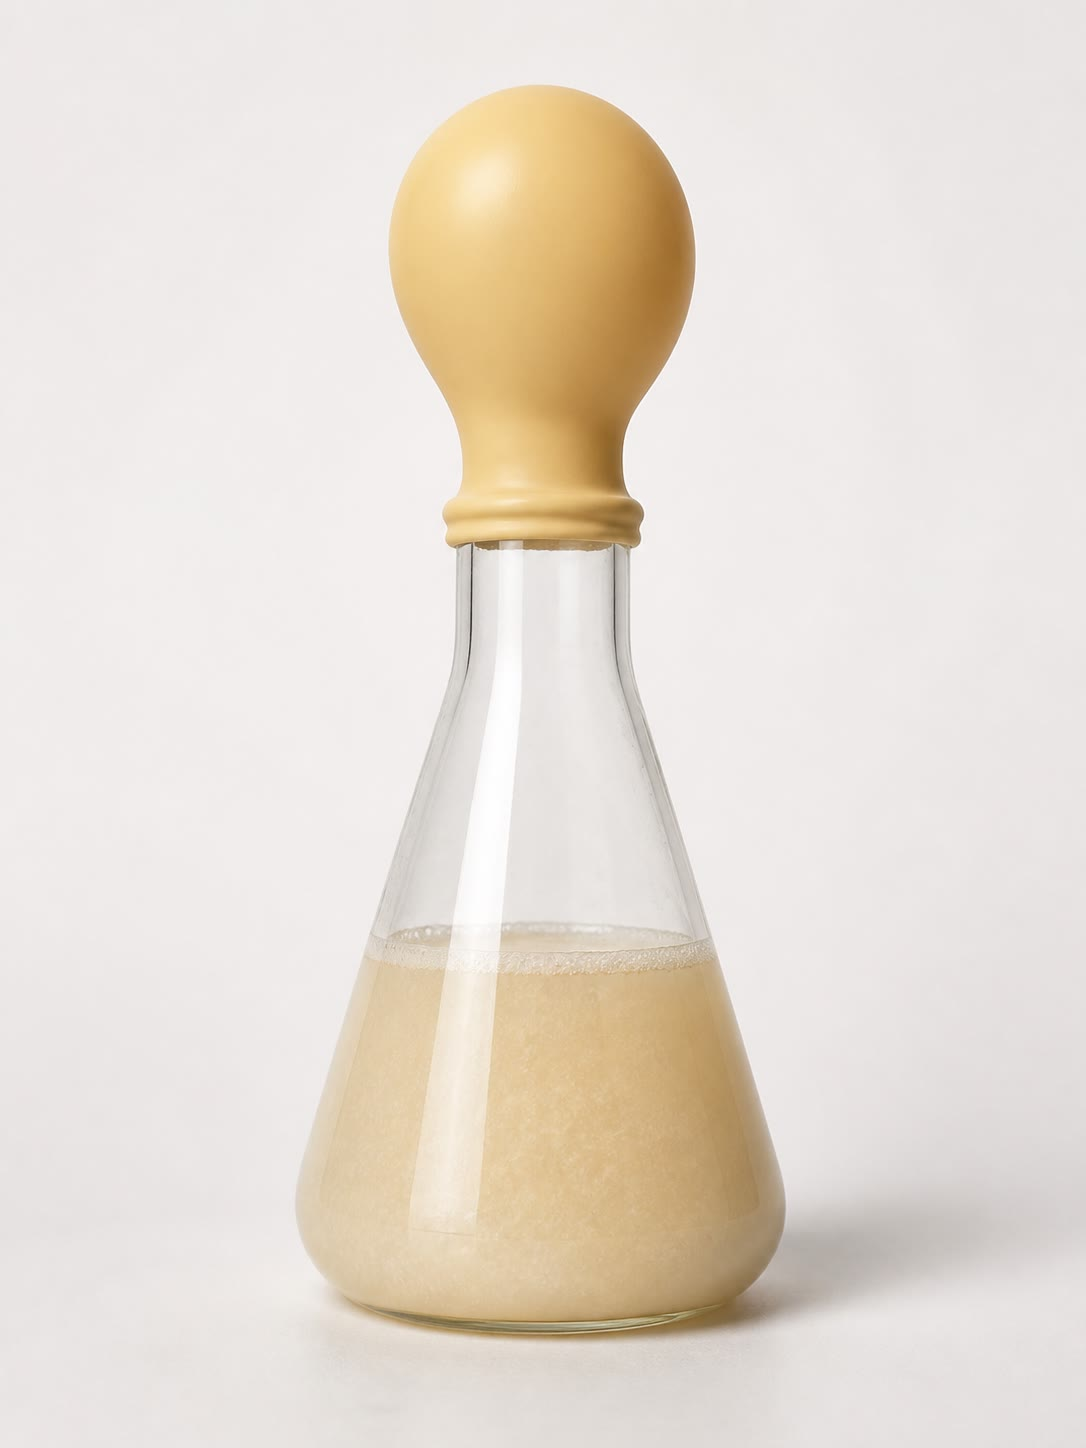
\includegraphics[width=0.36\linewidth]{images/book2/ai/g10-metab-yeast-balloon.jpg}

{\small फ़्लास्क में चीनी का \omterm{def:g10:cell-metabolism:fermentation}{किण्वन} करता खमीर: ऐल्कोहॉली \omterm{def:g10:cell-metabolism:fermentation}{किण्वन} की कार्बन
डाइऑक्साइड गुब्बारे को फुला देती है। तरल में ऑक्सीजन न होने से चीनी केवल
आंशिक रूप से टूटती है और इथेनॉल पीछे रह जाता है।}
\end{omfigure}

\begin{example}[हवा में और हवा के बिना खमीर]\label{ex:g10:cell-metabolism:pasteur}
जिस खमीर में हवा के बुलबुले छोड़े जाएँ वह ग्लूकोज़ कम ख़र्च करता है और
तेज़ी से बढ़ता है: वह श्वसन करता है। वही खमीर बंद टंकी में ग्लूकोज़
लालच से ख़र्च करता है, कम बढ़ता है और इथेनॉल बनाता है: वह \omterm{def:g10:cell-metabolism:fermentation}{किण्वन} करता
है। पास्तर ने, जिन्होंने 1861 में इसका वर्णन किया, \omterm{def:g10:cell-metabolism:fermentation}{किण्वन} को
``हवा के बिना जीवन'' कहा था; \omterm{def:g10:cells-common-unit:cell}{कोशिकाएँ} अपना \omterm{def:g10:cell-metabolism:metabolism}{उपापचय} उसी पथ पर मोड़ लेती हैं
जिसकी उनका पर्यावरण छूट दे, और चूँकि \omterm{def:g10:cell-metabolism:fermentation}{किण्वन} प्रति ग्लूकोज़ इतनी कम ऊर्जा
देता है, इसलिए जीने के लिए उन्हें कहीं अधिक चीनी फूँकनी पड़ती है।
\end{example}

\begin{omfigure}
\begin{tikzpicture}[>=Stealth, font=\small,
  cell/.style={draw, rounded corners, thick, minimum height=1.5cm, text width=2.7cm, align=center},
  inp/.style={text width=2.3cm, align=right, anchor=east},
  outp/.style={text width=2.6cm, align=left, anchor=west}]
  \node[cell, fill=omMeth!12] (a) at (0,0) {\textbf{स्वपोषी कोशिका}\\ हरितलवक};
  \node[inp] (ai) at (-2.2,0) {$\mathrm{CO_2}$, $\mathrm{H_2O}$,\\ खनिज लवण,\\ \emph{प्रकाश}};
  \node[outp] (ao) at (2.2,0) {कार्बनिक पदार्थ\\ (ग्लूकोज़, मंड\dots)\\ $+ \mathrm{O_2}$};
  \draw[->] (ai) -- (a); \draw[->] (a) -- (ao);
  \node[cell, fill=omThm!10] (h) at (0,-3.2) {\textbf{कोई भी कोशिका}\\ सूत्रकणिकाएँ};
  \node[inp] (hi) at (-2.2,-3.2) {कार्बनिक पदार्थ\\ $+ \mathrm{O_2}$};
  \node[outp] (ho) at (2.2,-3.2) {$\mathrm{CO_2}$, $\mathrm{H_2O}$\\ $+$ ऊर्जा (ATP, ऊष्मा)};
  \draw[->] (hi) -- (h); \draw[->] (h) -- (ho);
  \node[anchor=west, font=\small\itshape] at (8.6,0) {प्रकाशसंश्लेषण};
  \node[anchor=west, font=\small\itshape] at (8.6,-3.2) {श्वसन};
  \draw[->, gray, thick] (4.6,-0.7) to[bend left=35] node[right, font=\scriptsize, text width=3.6cm, align=left, xshift=2pt] {कार्बनिक पदार्थ परपोषियों को, और ख़ुद स्वपोषी के श्वसन को भी खिलाता है} (4.6,-2.5);
\end{tikzpicture}

{\small \omterm{def:g10:cells-common-unit:cell}{कोशिका} के \omterm{def:g10:cell-metabolism:metabolism}{उपापचय} की दो धाराएँ। \omterm{def:g10:cell-metabolism:autotrophy}{प्रकाशसंश्लेषण} प्रकाश की ऊर्जा
\omterm{def:g10:chemistry-of-life:mineral-organic}{कार्बनिक पदार्थ} में संचित करता है; और हर \omterm{def:g10:cells-common-unit:cell}{कोशिका} में श्वसन उसे छोड़ देता
है। \omterm{def:g10:cell-metabolism:autotrophy}{स्वपोषी} दोनों चलाते हैं; \omterm{def:g10:cell-metabolism:autotrophy}{परपोषी} केवल दूसरी चलाते हैं और उन्हें
\omterm{def:g10:chemistry-of-life:mineral-organic}{कार्बनिक पदार्थ} खिलाना पड़ता है।}
\end{omfigure}

\section{कोशिका का उपापचय तय क्या करता है}

\begin{proposition}[जीन और पर्यावरण]\label{prop:g10:cell-metabolism:decides}
किसी \omterm{def:g10:cells-common-unit:cell}{कोशिका} का \omterm{def:g10:cell-metabolism:metabolism}{उपापचय} दो चीज़ों पर निर्भर है: उसके
\emph{साज़-सामान} पर --- यानी उन एंजाइमों और \omterm{def:g10:cells-common-unit:organelle}{कोशिकांगों} पर जिन्हें उसके
\omterm{def:g10:universal-dna:gene}{जीन} बनाने देते हैं, इसलिए बिना पर्णहरित वाली \omterm{def:g10:cells-common-unit:cell}{कोशिका} कभी \omterm{def:g10:cell-metabolism:autotrophy}{प्रकाशसंश्लेषण}
नहीं कर सकती --- और उसके \emph{पर्यावरण} पर --- प्रकाश, ऑक्सीजन, उपलब्ध
पोषक तत्व --- जो तय करता है कि संभव पथों में से असल में कौन-सा चलेगा।
खमीर हवा में श्वसन करता है और उसके बिना \omterm{def:g10:cell-metabolism:fermentation}{किण्वन}; \emph{Euglena} प्रकाश में
\omterm{def:g10:cell-metabolism:autotrophy}{स्वपोषी} है और अँधेरे में \omterm{def:g10:cell-metabolism:autotrophy}{परपोषी}; और किसी हरे पौधे की जड़ की \omterm{def:g10:cells-common-unit:cell}{कोशिका} जीवन
भर \omterm{def:g10:cell-metabolism:autotrophy}{परपोषी} रहती है, जिसे पत्तियाँ खिलाती हैं।
\end{proposition}
\admitted

\begin{method}[उपापचय का आलेख पढ़ना]\label{met:g10:cell-metabolism:trace}
ऑक्सीजन संवेदक के प्रयोग समय के सापेक्ष सांद्रता देते हैं।
\begin{enumerate}
  \item पहचानिए कि हर चिह्नित क्षण पर क्या बदला (प्रकाश जला, क्रियाधार
        मिलाया गया, ऑक्सीजन चुक गई)।
  \item हर सीधे खंड की ढाल पढ़िए: उठान बटा दौड़, \unit{mg/L} प्रति मिनट
        में। धनात्मक ढाल का अर्थ है ऑक्सीजन का शुद्ध उत्पादन, ऋणात्मक का
        शुद्ध उपभोग।
  \item याद रखिए कि \omterm{def:g10:cell-metabolism:autotrophy}{प्रकाशसंश्लेषण} करती \omterm{def:g10:cells-common-unit:cell}{कोशिका} श्वसन भी करती है: प्रकाश
        में मिलने वाली ढाल उत्पादन में से श्वसन घटाकर बची ढाल है, इसलिए
        \omterm{def:g10:cell-metabolism:autotrophy}{प्रकाशसंश्लेषण} की सच्ची दर प्रकाश वाली ढाल में अँधेरे वाली ढाल
        का परिमाण जोड़ने से मिलती है।
  \item पूछा जाए तो बदल भी दीजिए: इन सांद्रताओं पर घुली हुई ऑक्सीजन का
        \qty{1}{mg/L} प्रति लीटर $1/32$ मिलीमोल है।
\end{enumerate}
\end{method}

\begin{example}[शैवाल की सच्ची दर]\label{ex:g10:cell-metabolism:truerate}
\emph{Chlorella} वाले चित्र में प्रकाश के 5 मिनट में ऑक्सीजन
\qty{2.5}{mg/L} बढ़ती है (ढाल $+0.5$) और अँधेरे के 5 मिनट में
\qty{0.5}{mg/L} घटती है (ढाल $-0.1$)। श्वसन प्रकाश में भी प्रति मिनट
\qty{0.1}{mg/L} खपाता है, इसलिए \omterm{def:g10:cell-metabolism:autotrophy}{प्रकाशसंश्लेषण} प्रति मिनट
$0.5 + 0.1 = \qty{0.6}{mg/L}$ बनाता है: यानी श्वसन के ख़र्च का छह गुना।
शैवाल ऑक्सीजन और \omterm{def:g10:chemistry-of-life:mineral-organic}{कार्बनिक पदार्थ} की शुद्ध उत्पादक है, और इसीलिए वह
बढ़ती है।
\end{example}

\section{अभ्यास}

\begin{exercise}[$\star$]\label{exo:g10:cell-metabolism:1}
\omterm{def:g10:cell-metabolism:metabolism}{उपापचय} की परिभाषा दीजिए, और बताइए कि \omterm{def:g10:cell-metabolism:metabolism}{एंजाइम} क्या है और क्या करता है।
\end{exercise}

\begin{exercise}[$\star$]\label{exo:g10:cell-metabolism:2}
\omterm{prop:g10:cell-metabolism:respiration}{कोशिकीय श्वसन} और \omterm{def:g10:cell-metabolism:autotrophy}{प्रकाशसंश्लेषण} के संक्षिप्त समीकरण लिखिए। किस अर्थ में
एक दूसरे का उल्टा है, और किस अर्थ में नहीं?
\end{exercise}

\begin{exercise}[$\star$]\label{exo:g10:cell-metabolism:3}
\omterm{def:g10:cell-metabolism:autotrophy}{स्वपोषी} या \omterm{def:g10:cell-metabolism:autotrophy}{परपोषी} में छाँटिए: एक कुकुरमुत्ता, एक मॉस, गाजर की जड़ की एक
\omterm{def:g10:cells-common-unit:cell}{कोशिका}, एक क्लोरेला, दही का एक जीवाणु, मनुष्य की एक पेशी \omterm{def:g10:cells-common-unit:cell}{कोशिका}।
\end{exercise}

\begin{exercise}[$\star$]\label{exo:g10:cell-metabolism:4}
खमीर और गुब्बारे वाले प्रयोग में गुब्बारे को कौन-सी गैस फुलाती है, कौन-सा
तरल उत्पाद जमा होता है, और फ़्लास्क में किस चीज़ की कमी है जो परिणाम बदल
देती?
\end{exercise}

\begin{exercise}[$\star$]\label{exo:g10:cell-metabolism:5}
उबला हुआ यकृत हाइड्रोजन परॉक्साइड में झाग क्यों नहीं उठाता?
\end{exercise}

\begin{exercise}[$\star\star$]\label{exo:g10:cell-metabolism:6}
खमीर वाले चित्र में मिनट 3 और 10 के बीच ऑक्सीजन \qty{7.9}{mg/L} से
\qty{0.9}{mg/L} तक गिरती है। श्वसन की दर \unit{mg/L} प्रति मिनट में
निकालिए। मिनट 10 के बाद वक्र चपटा क्यों पड़ जाता है, और खमीर तब क्या
करता है?
\end{exercise}

\begin{exercise}[$\star\star$]\label{exo:g10:cell-metabolism:7}
प्रकाश में क्लोरेला की ऑक्सीजन-ढाल $+0.8$ \unit{mg/L} प्रति मिनट है,
और अँधेरे में $-0.2$। \omterm{def:g10:cell-metabolism:autotrophy}{प्रकाशसंश्लेषण} की दर निकालिए।
\end{exercise}

\begin{exercise}[$\star\star$]\label{exo:g10:cell-metabolism:8}
कोई \omterm{def:g10:cells-common-unit:cell}{कोशिका} \qty{18}{g} ग्लूकोज़ का श्वसन करती है। वह ऑक्सीजन का कितना
द्रव्यमान इस्तेमाल करती है और कार्बन डाइऑक्साइड का कितना छोड़ती है?
(मोलर द्रव्यमान: ग्लूकोज़ \qty{180}{g/mol}, $\mathrm{O_2}$
\qty{32}{g/mol}, $\mathrm{CO_2}$ \qty{44}{g/mol}।)
\end{exercise}

\begin{exercise}[$\star\star$]\label{exo:g10:cell-metabolism:9}
निर्वात फ़्लास्क में अंकुरित होते मटर उसका ताप दिन भर में
\qty{4}{\celsius} बढ़ा देते हैं; उबले हुए मटर नहीं। दोनों परिणाम
समझाइए, और यह भी कि फ़्लास्क को हवाबंद क्यों नहीं करना चाहिए।
\end{exercise}

\begin{exercise}[$\star\star$]\label{exo:g10:cell-metabolism:10}
किसी हरे पत्ते को 48 घंटे अँधेरे में रखा जाता है, फिर उसका आधा हिस्सा
काले काग़ज़ से ढँककर पौधे को दिन भर धूप में रखा जाता है। फिर आयोडीन
लगाया जाता है। दोनों हिस्सों का परिणाम अनुमानित कीजिए और समझाइए, और यह भी
कि 48 घंटे के अँधेरे की ज़रूरत क्यों थी।
\end{exercise}

\begin{exercise}[$\star\star$]\label{exo:g10:cell-metabolism:11}
समझाइए कि बंद टंकी में रखा खमीर, प्रति \omterm{def:g10:cells-common-unit:cell}{कोशिका}, हवा के बुलबुलों वाले खमीर
से कहीं तेज़ी से चीनी क्यों खपाता है।
\end{exercise}

\begin{exercise}[$\star\star\star$]\label{exo:g10:cell-metabolism:12}
400 मीटर की दौड़ के बाद किसी धावक की पेशियाँ दुखने लगती हैं और अम्लीय हो
जाती हैं। समझाइए कि पेशी \omterm{def:g10:cells-common-unit:cell}{कोशिकाओं} में क्या हुआ, वह क्यों हुआ, और उसी
धावक की पेशियाँ धीमी जॉगिंग में अम्लीय क्यों नहीं होतीं।
\end{exercise}

\begin{exercise}[$\star\star\star$]\label{exo:g10:cell-metabolism:13}
कार्बनिक भोजन के साथ महीने भर अँधेरे में रखी \emph{Euglena} अपने \omterm{def:g10:cells-common-unit:organelle}{हरितलवक}
खो देती है, पर उसके वंशज प्रकाश में उन्हें दोबारा पा लेते हैं।
\cref{prop:g10:cell-metabolism:decides} के दोनों कारकों में से कौन-सा
बदला है और कौन-सा नहीं? उनका दोबारा बन जाना \omterm{def:g10:cells-common-unit:cell}{कोशिका} के \omterm{def:g10:universal-dna:gene}{जीनों} के बारे में
क्या सिद्ध करता है?
\end{exercise}

\begin{exercise}[$\star\star\star$]\label{exo:g10:cell-metabolism:14}
किसी बंद मछलीघर में पानी, एक घोंघा और एक जलीय पौधा है, और वह प्रकाश में
रखा है। समझाइए कि दोनों जीव महीनों तक कैसे बचे रह सकते हैं, हर एक दूसरे
को क्या देता है, और मछलीघर को अँधेरे में रखने पर क्या होता है।
\end{exercise}

\begin{exercise}[$\star\star\star$]\label{exo:g10:cell-metabolism:15}
एक ग्लूकोज़ के श्वसन से लगभग 30 ATP मिलते हैं, \omterm{def:g10:cell-metabolism:fermentation}{किण्वन} से 2। खमीर की एक
\omterm{def:g10:cells-common-unit:cell}{कोशिका} को जीने के लिए प्रति मिनट तय संख्या में ATP चाहिए। निकालिए कि
\omterm{def:g10:cell-metabolism:fermentation}{किण्वन} करते समय उसे प्रति मिनट कितने गुना अधिक ग्लूकोज़ खपाना पड़ेगा;
फिर समझाइए कि शराब बनाने वाले अपनी टंकियों से हवा क्यों बाहर रखते हैं,
जबकि इससे चीनी ``बरबाद'' होती है।
\end{exercise}

\section{समस्या: शराब बनाने वाले की टंकी}

\begin{problem}[{सप्ताहांत समस्या --- अंगूर के रस की एक टंकी खमीर के
हवाले: उसमें कितनी ऐल्कोहॉल बनेगी, कितनी गैस छूटेगी, कितनी ऊष्मा बनेगी,
और कोई तहख़ाना ख़तरनाक जगह क्यों हो सकता है}]
\label{pb:g10:cell-metabolism:1}
अंगूर के रस में प्रति लीटर लगभग \qty{200}{g} शर्करा होती है, जिसे हम
ग्लूकोज़ मानते हैं, और टंकी बंद कर देने के बाद उसमें घुली हुई ऑक्सीजन
नहीं रहती। मोलर द्रव्यमान: ग्लूकोज़ \qty{180}{g/mol}, इथेनॉल
$\mathrm{C_2H_5OH}$ \qty{46}{g/mol}, कार्बन डाइऑक्साइड \qty{44}{g/mol},
ऑक्सीजन \qty{32}{g/mol}। इथेनॉल का घनत्व \qty{0.79}{g/mL} है। तहख़ाने के
ताप पर एक मोल गैस लगभग \qty{24}{L} घेरती है। टंकी \qty{1000}{L} की है।

\medskip
\noindent\textbf{भाग I --- खमीर बनाता क्या है।}
\begin{enumerate}
  \item बंद टंकी में खमीर कौन-सा पथ चुनता है, और क्यों? उसका समीकरण
        लिखिए।
  \item एक लीटर रस में ग्लूकोज़ के कितने मोल हैं?
  \item प्रति लीटर बनने वाले इथेनॉल का द्रव्यमान निकालिए, फिर उसका
        आयतन, फिर शराब में आयतन के हिसाब से ऐल्कोहॉल की मात्रा प्रतिशत
        में।
  \item प्रति लीटर रस से बनने वाली कार्बन डाइऑक्साइड का द्रव्यमान
        निकालिए, और गैस के रूप में उसका आयतन भी।
  \item पूरी टंकी से कार्बन डाइऑक्साइड का कितना आयतन छूटता है?
        \qty{4}{m} गुणा \qty{6}{m} गुणा \qty{2.5}{m} के एक तहख़ाने के
        आयतन से तुलना कीजिए।
\end{enumerate}

\medskip
\noindent\textbf{भाग II --- अगर खमीर को हवा मिलती।}
\begin{enumerate}[resume]
  \item यदि रस में लगातार हवा भरी जाती तो खमीर जिस समीकरण पर चलता, वह
        लिखिए।
  \item एक लीटर रस की शर्करा का श्वसन करने के लिए ज़रूरी ऑक्सीजन का
        द्रव्यमान निकालिए, और छूटने वाली कार्बन डाइऑक्साइड का भी।
  \item प्रश्न 7 की कार्बन डाइऑक्साइड की तुलना प्रश्न 4 वाली से कीजिए,
        और ग्लूकोज़ कितनी दूर तक टूटता है, इसके आधार पर अंतर समझाइए।
  \item श्वसन प्रति ग्लूकोज़ लगभग 30 ATP देता है और \omterm{def:g10:cell-metabolism:fermentation}{किण्वन} 2। यदि खमीर
        को दोनों हालों में उतने ही ATP चाहिए, तो शर्करा किस हाल में
        अधिक चलेगी, और कितने गुना?
  \item समझाइए कि फिर भी शराब बनाने वाला हवा को बाहर क्यों रखता है।
\end{enumerate}

\medskip
\noindent\textbf{भाग III --- टंकी की ऊष्मा।}
\omterm{def:g10:cell-metabolism:fermentation}{किण्वन} प्रति मोल ग्लूकोज़ लगभग \qty{70}{kJ} ऊष्मा छोड़ता है; और
\qty{1}{kg} जल को \qty{1}{\celsius} गरम करने में \qty{4.2}{kJ} लगते हैं।
\begin{enumerate}[resume]
  \item प्रति लीटर रस से छूटने वाली ऊष्मा निकालिए, फिर पूरी टंकी के
        लिए।
  \item यदि उसमें से कुछ भी बाहर न निकले, तो टंकी का ताप कितना बढ़ेगा?
        (रस को जल मान लीजिए।)
  \item खमीर के \omterm{def:g10:cell-metabolism:metabolism}{एंजाइम} लगभग \qty{40}{\celsius} से ऊपर नष्ट हो जाते हैं।
        \qty{20}{\celsius} से शुरू करके क्या बिना ठंडा की गई टंकी बची
        रहेगी? इससे आपको क्या पता चलता है कि बड़ी टंकियाँ ठंडी क्यों की
        जाती हैं?
  \item \cref{prop:g10:cell-metabolism:enzymes} की मदद से समझाइए कि
        शर्करा अब भी मौजूद होने के बावजूद ऊष्मा \omterm{def:g10:cell-metabolism:fermentation}{किण्वन} को क्यों रोक
        देती है।
  \item श्वसन ने प्रति मोल लगभग \qty{2870}{kJ} छोड़े होते। जो ऊर्जा
        \omterm{def:g10:cell-metabolism:fermentation}{किण्वन} \emph{नहीं} छोड़ता, वह कहाँ बची रह जाती है?
\end{enumerate}

\medskip
\noindent\textbf{भाग IV --- तहख़ाना।}
\begin{enumerate}[resume]
  \item कार्बन डाइऑक्साइड हवा से सघन है। वह तहख़ाने में कहाँ जमा होती
        है, और नीचे तक ले जाई गई जलती मोमबत्ती एक परंपरागत सुरक्षा
        परीक्षण क्यों है?
  \item ऑक्सीजन से वंचित किसी मज़दूर की \omterm{def:g10:cells-common-unit:cell}{कोशिकाएँ} किस पथ पर चली जातीं ---
        और मानव शरीर उस पर कुछ मिनटों से अधिक क्यों नहीं जी सकता?
  \item ऐल्कोहॉल के आयतन के हिसाब से लगभग 15\% पहुँचते ही \omterm{def:g10:cell-metabolism:fermentation}{किण्वन} अपने आप
        रुक जाता है। खमीर के एंजाइमों के आधार पर इसका एक स्पष्टीकरण
        सुझाइए।
  \item ब्रेड का गुँधा आटा उसी खमीर को एक घंटे इस्तेमाल करता है। गूदे के
        बुलबुलों में क्या है, और सिंकने के बाद इथेनॉल कहाँ चला जाता है?
  \item परिणाम लिखिए: एक लीटर रस के लिए ऐल्कोहॉल की मात्रा और बनी हुई
        गैस का आयतन --- और वह अकेला उपापचयी तथ्य जो दोनों को समझा देता
        है।
\end{enumerate}
\end{problem}
